\pagebreak
\subsection{Ground Support Equipment}\label{sec:4.9}
The purpose of the ground station is to monitor in real-time the experiment and provide manual override capability in case the experiment failed functioning autonomously. The manual override is able to control all the valves, pump, and heaters. \par
One personal computer will be used to connect to the E-Link through the Ethernet port. A GUI is created to display the sensors data and valves, pump states during the experiment. MATLAB GUIDE is used for the development. \par
The design of the ground station is responsible for receiving and transmitting data over the provided Ethernet connection. Using GUIDE to create a GUI and respective functions as a skeleton, the necessary  functionality to receive, transmit and display are built accordingly. The functions are defined for each GUI element.
\begin{figure}[H]
    \centering
    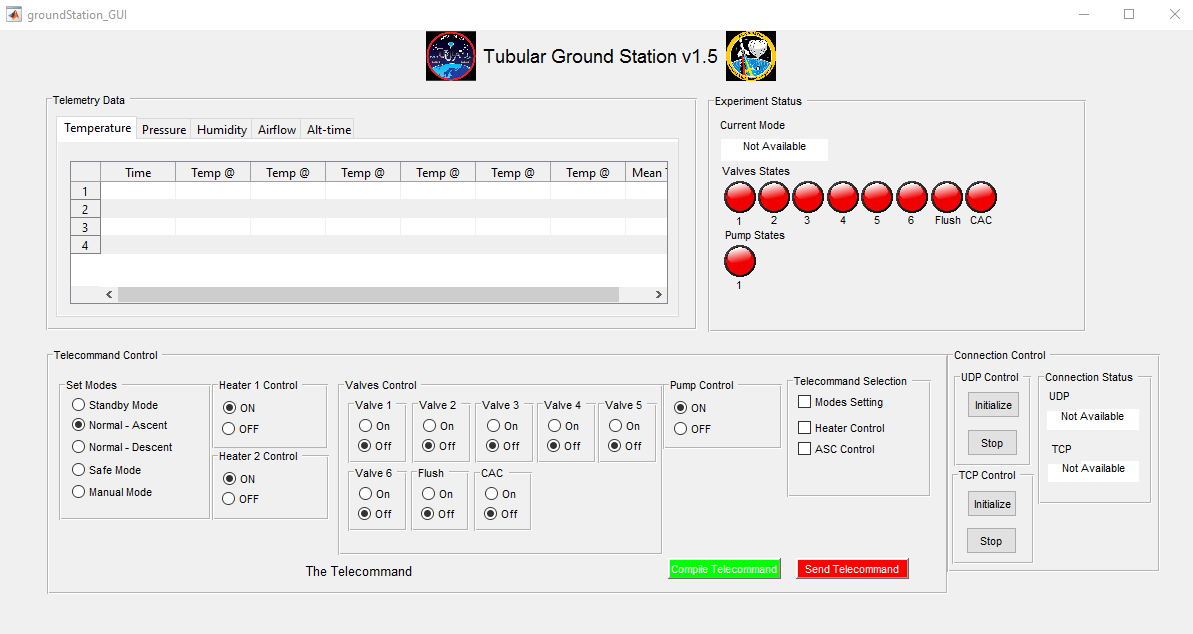
\includegraphics[width=0.8\textwidth]{4-experiment-design/img/GS-GUI2.png}
    \caption{GUI Design for Ground Station Version 1.5}
    \label{fig:guiDesign}
\end{figure}
Figure \ref{fig:guiDesign} shows current design of ground station GUI. Telemetry data will be shown in several tables based on the data type. The data shall be recorded and stored on the computer. The experiment status panel represents the real-time status of the experiments, the red indicator will change to green indicator if the pump or valves are open later on. On the bottom side, the telecommand control panel provides command generation for the experiment. On its right side, connection control panel has full control of the connections.


\raggedbottom